% 导入配置
% \documentclass[lang = cn, scheme = chinese, thmcnt = section]{elegantbook}
% elegantbook      设置elegantbook文档类
% lang = cn        设置中文环境
% scheme = chinese 设置标题为中文
% thmcnt = section 设置计数器


%% 1.封面设置

\title{Algebra Chapter 0 - Paolo Aluffi - NoteBook}                % 文档标题

\author{若水}               % 作者

\myemail{ethanmxzhou@163.com} % 邮箱

\homepage{helloethanzhou.github.io} % 主页

\date{\today}               % 日期

\extrainfo{上善若水任方圆}   % 箴言

\logo{PiCreatures_happy.pdf}        % 设置Logo

\cover{阿基米德螺旋曲线.pdf}          % 设置封面图片

% 修改标题页的色带
\definecolor{customcolor}{RGB}{135, 206, 250} 
% 定义一个名为customcolor的颜色,RGB颜色值为(135, 206, 250)

\colorlet{coverlinecolor}{customcolor}     % 将coverlinecolor颜色设置为customcolor颜色

%% 2.目录设置
\setcounter{tocdepth}{3}  % 目录深度为3

%% 3.引入宏包
\usepackage[all]{xy}
\usepackage{bbm, svg, graphicx, float, extpfeil, amsmath, amssymb, mathrsfs, mathalpha, boondox-cal, boondox-calo, hyperref, graphicx, romannum, chemarrow, booktabs, fontspec, ctex}

%% 4.定义命令
\newcommand{\N}{\mathbb{N}}            % 自然数集合
\newcommand{\R}{\mathbb{R}}            % 实数集合
\newcommand{\C}{\mathbb{C}}  		   % 复数集合
\newcommand{\Q}{\mathbb{Q}}            % 有理数集合
\newcommand{\Z}{\mathbb{Z}}            % 整数集合
\newcommand{\F}{\mathbb{F}}
\newcommand{\sub}{\subset}             % 包含
\newcommand{\im}{\text{im }}           % 像
\newcommand{\lang}{\langle}            % 左尖括号
\newcommand{\rang}{\rangle}            % 右尖括号
\newcommand{\dis}{\displaystyle}
\newcommand{\cont}{\text{cont}}
\newcommand{\cha}{\text{char}}
\newcommand{\function}[5]{
	\begin{align*}
		#1:\begin{aligned}[t]
			#2 &\longrightarrow #3\\
			#4 &\longmapsto #5
		\end{aligned}
	\end{align*}
}                                     % 函数

\newcommand{\lhdneq}{%
	\mathrel{\ooalign{$\lneq$\cr\raise.22ex\hbox{$\lhd$}\cr}}} % 真正规子群

\newcommand{\rhdneq}{%
	\mathrel{\ooalign{$\gneq$\cr\raise.22ex\hbox{$\rhd$}\cr}}} % 真正规子群

\newcommand{\upiff}{\mathrel{\rotatebox[origin=c]{90}{$\iff$}}} % 竖着的等价

\newcommand{\Rmnum}[1]{\uppercase\expandafter{\romannumeral #1}}  %定义命令输入大写罗马数字
\newcommand{\rmnum}[1]{\romannumeral #1}  %定义命令输入小写罗马数字



% \begin{document}

\chapter{域论}

\section{域扩张$\rm\Rmnum{1}$}

\subsection{基本定义}

\subsubsection{域扩张}

\begin{definition}{$\textsf{Fld}$范畴}
	\begin{enumerate}
		\item 对象:$\text{Obj}(\textsf{Fld})=\{ \text{域} F \}$
		\item 态射:$\text{Hom}_{\textsf{Fld}}(F,K)=\{ \text{环同态映射 }\varphi:F\to K \}$
	\end{enumerate}
\end{definition}

\begin{definition}{域扩张 field extension}
	对于域$k$与$K$,称$K/k$为域扩张,如果存在同态映射$\varphi:k\to K$。
\end{definition}

\begin{definition}{扩域 extend field}
	对于域扩张$K/k$,称$K$为$k$的扩域。
\end{definition}

\begin{definition}{子域 subfield}
	对于域扩张$K/k$,称$k$为$K$的子域。
\end{definition}

\begin{definition}{中间域 intermediate field}
	对于域扩张$k\sub F \sub K$,称$F$为$K/k$的中间域。
\end{definition}

\begin{proposition}{}{域间的同态映射为单射}
	对于域扩张$K/k$,其同态映射$\varphi:k\hookrightarrow K$为单射。
\end{proposition}

\begin{proof}
	由命题\ref{cor:域同态映射为单射},命题得证!
\end{proof}

\subsubsection{域的特征}

\begin{definition}{特征 characteristic}
	\begin{enumerate}
		\item 对于域$F$,存在且存在唯一同态映射
		\function{\varphi}{\Z}{F}{n}{n1_F}
		令$\ker\varphi=p\Z$,定义域$F$的特征为$\cha(F)=p$。
		\item 定义域$F$的特征为乘法单位元$1$在加法群$(F,+)$中的阶,并记作$\cha(F)$;特别的,如果乘法单位元$1$在加法群$(F,+)$中的阶为$\infty$,那么$\cha(F)=0$。
		\item 定义域$F$的特征为
		$$
		\cha(F)=\begin{cases}
			\min\{ n\in\N^*:nx=0,\forall x\in F \},\quad & \exists n\in\N^*,\forall x\in F,nx=0\\
			0,\quad & \forall n\in\N^*,\exists x\in F,nx\ne0
		\end{cases}
		$$
	\end{enumerate}
\end{definition}

\begin{proposition}{域的特征为零或素数}{域的特征为零或素数}
	对域$K$,或$\cha(F)=0$,或$\cha(F)$为素数。
\end{proposition}

\begin{proof}
	如果域$F$的特征$p=\cha(F)$成立$p\ne 0$且$p$不为素数,那么存在$m,n\ge 2$,使得成立$p=mn$。而%
	$$
	0=p1_F=(mn)1_F=(m1_F)\cdot (n1_F)
	$$
	由消去律,$m1_F=0$或$n1_F=0$,矛盾!
\end{proof}

\begin{proposition}{}{域扩张的特征相等}
	对于域扩张$K/k$,成立$\cha(k)=\cha(K)$。
\end{proposition}

\begin{proof}
	 对于同态映射%
	 $$
	 i:k\hookrightarrow K,\qquad 
	 \varphi:\Z\to k,\qquad
	 \psi:\Z\to K
	 $$
	 其中$\psi=i\circ \varphi$,考察其核,由命题\ref{pro:环的单态射}
	 \begin{align*}
	 	n\in \ker\psi
	 	& \iff \psi(n)=0_K\\
	 	& \iff (i\circ \varphi)(n)=0_K\\
	 	& \iff i(\varphi(n))=0_K\\
	 	& \iff \varphi(n)=n_k\\
	 	& \iff n\in \ker\varphi
	 \end{align*}
 	因此$\ker\varphi=\ker\psi$,进而$\cha(k)=\cha(K)$。
\end{proof}

\begin{definition}{$\textsf{Fld}_0$范畴}
	\begin{enumerate}
		\item 对象:$\text{Obj}(\textsf{Fld})=\{ \text{域} F:\cha(F)=0 \}$
		\item 态射:$\text{Hom}_{\textsf{Fld}}(F,K)=\{ \text{环同态映射 }\varphi:F\to K \}$
	\end{enumerate}
\end{definition}

\begin{definition}{$\textsf{Fld}_p$范畴}
	\begin{enumerate}
		\item 对象:$\text{Obj}(\textsf{Fld})=\{ \text{域} F:\cha(F)=p \}$
		\item 态射:$\text{Hom}_{\textsf{Fld}}(F,K)=\{ \text{环同态映射 }\varphi:F\to K \}$
	\end{enumerate}
\end{definition}

\begin{proposition}{$\textsf{Fld}_0$的初始对象}
	$\textsf{Fld}_0$的初始对象为$\Q$;换言之,对于任意特征为$0$的域$F$,存在且存在唯一同态映射$\varphi:\Q\hookrightarrow F$。
\end{proposition}

\begin{proposition}{$\textsf{Fld}_p$的初始对象}
	$\textsf{Fld}_p$的初始对象为$\F_p=\Z/p\Z$;换言之,对于任意特征为$p$的域$F$,存在且存在唯一同态映射$\varphi:\F_p\hookrightarrow F$。
\end{proposition}

\subsection{单扩张}

\subsubsection{单扩张结构}

\begin{definition}{生成域}{生成域}
	对于域扩张$K/k$,定义域$k$关于集合$S\sub K$的生成域为%
	$$
	k(S)=\bigcap_{F\supset k\cup S\text{ 为域}}F
	$$
\end{definition}

\begin{definition}{有理多项式域}
	对于域$F$,定义其有理多项式域为由多项式整环$F[x]$生成的分式域,即
	$$
	F(x)=\left\{ \frac{\dis\sum_{k=0}^{n}a_kx^k}{\dis\sum_{k=0}^{m}b_kx^k}:a_k,b_k\in F,m,n\in\N \right\}
	$$
\end{definition}

\begin{definition}{单扩张 simple extension}
	称域扩张$K/k$为单扩张,如果存在$\alpha\in K$,使得成立$K=k(\alpha)$。
\end{definition}

\begin{definition}{极小多项式 minimal polynomial}
	对于域扩张$K/k$,称$k$的代数元$\alpha$的极小多项式为$p(x)\in k[x]$,如果$p(\alpha)=0$,且$p(x)$为在$k[x]$中不可约的首一多项式。
\end{definition}

\begin{lemma}{}{极小多项式引理1}
	对于域扩张$k\sub K\sub F$,令$p(x)\in k[x]$为$\alpha\in F$在$k$上的极小多项式,令$P(x)\in K[x]$为$\alpha$在$K$上的极小多项式,那么$P(x)\mid p(x)$。
\end{lemma}

\begin{theorem}{单扩张结构}{单扩张结构}
	对于域扩张$K/k$,考虑$\alpha\in K$生成的单扩张$k(\alpha)/k$,令映射
	\function{\varphi}{k[t]}{k(\alpha)}{f(t)}{f(\alpha)}
	那么成立如下命题。
	\begin{enumerate}
		\item $\varphi\text{ 为单射}\iff \ker\varphi=\{0\}\iff[k(\alpha):k]=\infty$
		\item 当$\varphi$为单射时,$k(t)\cong k(\alpha)$。
		\item 当$\varphi$不为单射时,令$p(t)$为$\alpha$的极小多项式,则$\deg(p(x))=[k(\alpha):k]$,且$k[t]/(p(t))\cong k(\alpha)$。
	\end{enumerate}
\end{theorem}

\begin{proof}
	由命题\ref{pro:环的单态射}%
	$$
	\varphi\text{ 为单射}\iff \ker\varphi=\{0\}
	$$
	
	如果$\ker\varphi=\{0\}$,那么$\varphi$为单射。由命题\ref{pro:多项式整环},$k[t]$为整环。由分式域的万有性质\ref{def:分式域},存在且存在唯一同态映射$\psi:k(t)\to k(\alpha)$,使得成立
	$$
	\xymatrix{
		k(t) \ar[rr]^{\psi}  & & k(\alpha) \\
		& k[t] \ar@{^(->}[ul]^{i} \ar@{_(->}[ur]_{\varphi}
	}
	$$
	因此$\varphi:k[t]\to k(\alpha)$诱导同态映射
	\function{\psi}{k(t)}{k(\alpha)}{f(t)}{f(\alpha)}
	由命题\ref{cor:域同态映射为单射},$\psi$为单射。由第一同构定理\ref{thm:环第一同构定理},$k(t)\cong \im\psi$,因此$\im\psi$为包含$k$与$\alpha$的最小域,那么$\im\psi=k(\alpha)$,进而$k(t)\cong k(\alpha)$。
	
	由于$\{ t^i \}_{i=1}^{\infty}$在$k(t)$中线性无关,那么$\{ \alpha^i \}_{i=1}^{\infty}$在$k(\alpha)$中线性无关,进而$[k(\alpha):k]=\infty$。
	
	如果$\ker\varphi\ne \{0\}$,那么由命题\ref{pro:环的单态射},$\varphi$不为单射。由命题\ref{pro:域的多项式环为PID},存在且存在唯一不可约的首一多项式$p(t)\in k[t]$,使得成立$\ker\varphi=(p(t))$。由第一同构定理\ref{thm:环第一同构定理},$k[t]/(p(t))\cong \im\varphi$。由命题\ref{pro:子环的像为子环},$\im\varphi$为$k(\alpha)$的子环。由命题\ref{pro:整环的非零子环},$\im\varphi$为整环,因此$k[t]/(p(t))$为整环,进而$(p(t))$为$k[t]$的素理想。由命题\ref{pro:F[x]的素理想与极大理想},$(p(t))$为$k[t]$的极大理想,因此$k[t]/(p(t))$为域,进而$\im\varphi$为$k(\alpha)$的子域。而$k\cup\{\alpha\}\sub\im\varphi$,因此$\im\varphi=k(\alpha)$,进而$k[t]/(p(t))\cong k(\alpha)$。
	
	而$\varphi(t)=\alpha$,且%
	$$
	p(t+(p(t)))=p(t)+(p(t))=(p(t))
	$$
	因此$p(\alpha)=0$,进而$p(t)$为$\alpha$的极小多项式。
\end{proof}

\begin{example}
	\begin{align*}
		& \Q(\sqrt{2})=\{ a+b\sqrt{2}:a,b\in\Q \}\\
		& \frac{Q[x]}{(x^2-2)}=\{ a+bx+(x^2-2):a,b\in\Q \}
	\end{align*}
\end{example}

\begin{example}
	\begin{align*}
		& \Q(\sqrt{3})=\{ a+b\sqrt{3}:a,b\in\Q \}\\
		& \frac{Q[x]}{(x^2-3)}=\{ a+bx+(x^2-3):a,b\in\Q \}
	\end{align*}
\end{example}

\begin{corollary}{单扩张的基}{单扩张的基}
	\begin{enumerate}
		\item 对于单扩张$k(\alpha)/k$,若$[k(\alpha):k]=\infty$,则$\{ \alpha^i \}_{i=0}^{\infty}$为域$k$上的向量空间$k(\alpha)$的基,此时
		$$
		k(\alpha)=\left\{ \sum_{i=0}^{\infty}a_i\alpha^i:a_i\in k,i\in\N \right\}
		$$
		\item 对于单扩张$k(\alpha)/k$,若$[k(\alpha):k]=n$,则$\{ \alpha^i \}_{i=0}^{n-1}$为域$k$上的向量空间$k(\alpha)$的基,此时
		$$
		k(\alpha)=\left\{ \sum_{i=0}^{n-1}a_i\alpha^i:a_i\in k,0\le i \le n-1 \right\}
		$$
	\end{enumerate}
\end{corollary}

\begin{proposition}{单扩张间的同构映射的延拓}{单扩张间的同构映射的延拓}
	对于单扩张$k_1(\alpha_1)/k_1$与$k_2(\alpha_2)/k_2$,令$p_1(t)\in k_1[t]$与$p_2(t)\in k_2[t]$分别为$\alpha_1$与$\alpha_2$的极小多项式,如果同构映射$i:k_1\to k_2$成立%
	$$
	i(p_1(t))=p_2(t)
	$$
	那么存在且存在唯一同构映射$j:k_1(\alpha_1)\to k_2(\alpha_2)$,使得成立$j|_{k_1}=i$,且$j(\alpha_1)=\alpha_2$。
\end{proposition}

\begin{proof}
	对于存在性,由于同构映射$i:k_1\to k_2$成$i(p_1(t))=p_2(t)$,那么其诱导同构映射%
	$$
	\frac{k_1[t]}{(p_1(t))}\xrightarrow{\sim}\frac{k_2[t]}{(p_2(t))}
	$$
	由单扩张结构\ref{thm:单扩张结构},给出%
	$$
	j:k_1(\alpha_1)
	\xrightarrow{\sim}\frac{k_1[t]}{(p_1(t))}
	\xrightarrow{\sim}\frac{k_2[t]}{(p_2(t))}
	\xrightarrow{\sim}k_2(\alpha_2)
	$$
	
	对于唯一性,如果存在同构映射$j':k_1(\alpha_1)\to k_2(\alpha_2)$,使得成立$j'_{k_1}=i$,且$j'(\alpha_1)=\alpha_2$,那么由单扩张的基\ref{cor:单扩张的基},令$n=\deg(p_1(t))$,则
	$$
	k(\alpha)=\left\{ \sum_{i=0}^{n-1}a_i\alpha^i:a_i\in k,0\le i \le n-1 \right\}
	$$
	由于
	$$
	j'\left(\sum_{i=0}^{n-1}a_i\alpha_1^i\right)
	=\sum_{i=0}^{n-1}j'(a_i)j'(\alpha_1)^i
	=\sum_{i=0}^{n-1}j(a_i)\alpha_2^i
	=\sum_{i=0}^{n-1}j(a_i)j(\alpha_1)^i
	=j\left(\sum_{i=0}^{n-1}a_i\alpha_1^i\right)
	$$
	因此$j'=j$。
\end{proof}

\begin{corollary}{}{单扩张间的同构映射的延拓的推论}
	对于单扩张$k_1(\alpha_1)/k_1$与$k_2(\alpha_2)/k_2$,如果同构映射$i:k_1\to k_2$保持极小多项式,那么$i$可唯一延拓为同构映射$j:k_1(\alpha_1)\to k_2(\alpha_2)$,且保持代数元。换言之
	$$
	\xymatrix{
		k_1(\alpha_1) \ar[r]^\sim_j & k_2(\alpha_2)\\
		k_1 \ar[r]^\sim_i \ar@{^(->}[u] & k_2 \ar@{_(->}[u]
	}
	$$
\end{corollary}

\subsubsection{$k$-自同构映射群}

\begin{definition}{$k$-同态映射}
	对于域扩张$K/k$与$F/k$,称同态映射$\varphi:K\to F$为$k$-同态映射,如果$\varphi|_k=\mathbbm{1}_k$。
\end{definition}

\begin{definition}{$k$-同构映射}
	对于域扩张$K/k$与$F/k$,称同构映射$\varphi:K\to F$为$k$-同构映射,如果$\varphi|_k=\mathbbm{1}_k$。
\end{definition}

\begin{definition}{$k$-自同构映射}
	对于域扩张$K/k$,称同构映射$\varphi:K\to K$为$k$-自同构映射,如果$\varphi|_k=\mathbbm{1}_k$。
\end{definition}

\begin{definition}{$k$-自同构映射群}
	对于域扩张$K/k$,$k$-自同构映射$\varphi:K\to K$全体依映射复合运算构成$k$-自同构映射群,记作$\text{Aut}_k(K)$。
\end{definition}

\begin{proposition}
	对于单扩张$k(\alpha)/k$,如果$p(x)\in k[x]$为$\alpha$的极小多项式,令$\text{Root}_p=\{ x\in k(\alpha):p(x)=0 \}$,那么成立等式%
	$$
	|\text{Aut}_k(k(\alpha))|=|\text{Root}_p|
	$$
	特别的,成立不等式
	$$
	|\text{Aut}_k(k(\alpha))|\le[k(\alpha):k]
	$$
	当且仅当$p(x)$可在$k(\alpha)$中分解为一次因式之积时等号成立。
\end{proposition}

\begin{proof}
	作映射
	\function{\mathscr{F}}{\text{Aut}_k(k(\alpha))}{\text{Root}_p}{\varphi}{\varphi(\alpha)}
	
	首先我们证明映射的定义良好性
	$$
	p(\varphi(\alpha))
	=\varphi(p(\alpha))
	=\varphi(0)
	=0
	$$
	
	其次我们证明$\mathscr{F}$为单射,任取$\varphi,\psi\in \mathscr{F}$,使得成立$\varphi(\alpha)=\psi(\alpha)$。由单扩张的基\ref{cor:单扩张的基},令$n=\deg(p(t))$,则
	$$
	k(\alpha)=\left\{ \sum_{i=0}^{n-1}a_i\alpha^i:a_i\in k,0\le i \le n-1 \right\}
	$$
	由于
	$$
	\varphi\left(\sum_{i=0}^{n-1}a_i\alpha^i\right)
	=\sum_{i=0}^{n-1}\varphi(a_i)\varphi(\alpha)^i
	=\sum_{i=0}^{n-1}a_i\varphi(\alpha)^i
	=\sum_{i=0}^{n-1}a_i\psi(\alpha)^i
	=\sum_{i=0}^{n-1}\psi(a_i)\psi(\alpha)^i
	=\psi\left(\sum_{i=0}^{n-1}a_i\alpha^i\right)
	$$
	因此$\varphi=\psi$。由$\varphi,\psi$的任意性,$\mathscr{F}$为单射。
	
	最后我们证明$\mathscr{F}$为满射,任取$\beta\in \text{Root}_p$,那么$p(x)$为$\beta$的极小多项式。由命题\ref{pro:单扩张间的同构映射的延拓},存在同构映射$\varphi:k(\alpha)\to k(\beta)$,使得成立$\varphi|_{k}=\mathbbm{1}_k$,且$\varphi(\alpha)=\beta$。由单扩张结构\ref{thm:单扩张结构}%
	$$
	k(\alpha)\cong\frac{k[x]}{(p(x))}\cong k(\beta)
	$$
	因此$\varphi\in \text{Aut}_k(k(\alpha))$,进而$\mathscr{F}(\varphi)=\beta$。由$\beta$的任意性,$\mathscr{F}$为满射。
	
	综合以上三点,成立等式%
	$$
	|\text{Aut}_k(k(\alpha))|=|\text{Root}_p|
	$$
	
	由定理\ref{thm:单扩张结构}与引理\ref{lem:n次多项式至多存在n个根}
	$$
	|\text{Aut}_k(k(\alpha))|
	=|\text{Root}_p|
	\le\dim(p(x))
	=[k(\alpha):k]
	$$
	显然当且仅当$p(x)$可在$k(\alpha)$中分解为一次因式之积时等号成立。
\end{proof}

\subsection{有限扩张与代数扩张}

\subsubsection{有限扩张}

\begin{definition}{向量空间 vector space}
	称$(V,+,\;\cdot\;)$为域$F$上的向量空间,如果加法运算$+:V\times V\to V$与数乘运算$\cdot:F\times V\to V$成立如下性质。
	\begin{enumerate}
		\item 加法单位元:存在$0\in V$,使得对于任意$x\in V$,成立$0+x=x+0=x$。
		\item 数乘单位元:存在$1\in F$,使得对于任意$x\in V$,成立$1\cdot x=x$。
		\item 加法逆元:对于任意$x\in V$,存在$y\in V$,使得成立$x+y=y+x=0$。
		\item 加法交换律:$x+y=y+x$
		\item 加法结合律:$x+(y+z)=(x+y)+z$
		\item 数乘结合律:$\lambda\cdot (\mu\cdot x)=(\lambda\mu)\cdot x$
		\item 数乘左分配律:$(\lambda+\mu)\cdot x=\lambda \cdot x+\mu \cdot x$
		\item 数乘右分配律:$\lambda\cdot(x+y)=\lambda \cdot x+\lambda \cdot y$
	\end{enumerate}
\end{definition}

\begin{definition}{域扩张的向量空间性}
	对于域扩张$K/k$,可将$K$看作$k$上的向量空间。
\end{definition}

\begin{definition}{扩张次数 degree of extension}
	对于域扩张$K/k$,将$K$看作$k$上的向量空间,定义域扩张的次数为$[K:k]=\dim(K)$。
\end{definition}

\begin{definition}{有限扩张 finite extension}
	称域扩张$K/k$为$n$次扩张,如果$[K:k]=n$。
\end{definition}

\begin{lemma}{}{扩张次数不等式1}
	对于域扩张$k\sub K\sub F$,成立$[F:k]\ge [K:k]$。
\end{lemma}

\begin{proof}
	若$[F:k]=\infty$,则命题显然成立。若$[F:k]<\infty$,则由望远镜定理\ref{pro:望远镜定理}%
	$$
	[F:k]=[F:K][K:k]\ge [K:k]
	$$
\end{proof}

\begin{lemma}{}{扩张次数不等式2}
	对于域扩张$k\sub K\sub F$,成立$[F:k]\ge [F:K]$。
\end{lemma}

\begin{proof}
	若$[F:k]=\infty$,则命题显然成立。若$[F:k]<\infty$,则由望远镜定理\ref{pro:望远镜定理}%
	$$
	[F:k]=[F:K][K:k]\ge [F:K]
	$$
\end{proof}

\begin{lemma}{}{扩张次数不等式3}
	对于域扩张$k\sub K\sub F$,令$\alpha\in F$,则$[k(\alpha):k]\ge [K(\alpha):K]$。
\end{lemma}

\begin{proof}
	若$[k(\alpha):k]=\infty$,则命题显然成立。若$[k(\alpha):k]<\infty$,则$\alpha$为$k$上的代数元。令$p(x)\in p[x]$为$\alpha$在$k$上的极小多项式。那么将$p(x)$看作$K[x]$中的多项式,从而$\alpha$为$K$上的代数元。令$P(x)\in K[x]$为$\alpha$在$K$上的极小多项式,由引理\ref{lem:极小多项式引理1},$P(x)\mid p(x)$,从而$\deg(P(x))\le \deg(p(x))$。由定理\ref{thm:单扩张结构}%
	$$
	[k(\alpha):k]
	=\deg(p(x))
	\ge \deg(P(x))
	=[K(\alpha):K]
	$$
\end{proof}

\subsubsection{代数扩张}

\begin{definition}{代数元 algebraic element}
	对于域扩张$K/k$,称$\alpha\in K$为$k$的代数元,如果成立如下命题之一。
	\begin{enumerate}
		\item $[k(\alpha):k]<\infty$
		\item 存在非常多项式$f(x)\in k[x]$,使得成立$f(\alpha)=0$。
	\end{enumerate}
\end{definition}

\begin{definition}{超越元 transcendantal element}
	对于域扩张$K/k$,称$\alpha\in K$为$k$的超越元,如果成立如下命题之一。
	\begin{enumerate}
		\item $[k(\alpha):k]=\infty$
		\item 对于任意非常多项式$f(x)\in k[x]$,成立$f(\alpha)\ne 0$。
	\end{enumerate}
\end{definition}

\begin{definition}{代数扩张 algebraic extension}{代数扩张}
	称域扩张$K/k$为代数扩张,如果对于任意$\alpha\in K$,$\alpha$为$k$的代数元。
\end{definition}

\begin{lemma}{有限扩张$\implies$代数扩张}{有限扩张implies代数扩张}
	如果域扩张$K/k$为有限扩张,那么$K/k$为代数扩张,且对于任意$\alpha\in K$,成立$[k(\alpha):k]\le [K:k]$。
\end{lemma}

\begin{proof}
	由于对于任意$\alpha\in K$,成立$k\sub k(\alpha)\sub K$,那么$[k(\alpha):k]\le [K:k]$,因此$K/k$为代数扩张。
\end{proof}

\begin{lemma}{有限单扩张$\iff$代数单扩张}{单扩张时有限扩张iff代数扩张}
	对于单扩张$k(\alpha)/k$,成立%
	$$
	k(\alpha)/k\text{ 为有限扩张}
	\iff k(\alpha)/k\text{ 为代数扩张}
	$$
\end{lemma}

\begin{proof}
	一方面,由引理\ref{lem:有限扩张implies代数扩张},若$k(\alpha)/k$为有限扩张,则$k(\alpha)/k$为代数扩张。
	
	另一方面,若$k(\alpha)/k$为代数扩张,则$\alpha$为代数元,因此$[k(\alpha):k]<\infty$,进而$k(\alpha)/k$为有限扩张。
\end{proof}

\begin{proposition}{望远镜定理}{望远镜定理}
	对于域$F\sub L\sub K$,成立
	$$
	[K:F]<\infty\iff [K:L]<\infty\text{且}[L:F]<\infty
	$$
	此时成立
	$$
	[K:F]=[K:L][L:F]
	$$
\end{proposition}

\begin{proof}
	对于必要性,如果$[K:F]=n$,那么由于$L$为$K$的子空间,因此$[L:F]\le n$。设$\{\alpha_k\}_{k=1}^{n}$为向量空间$K/F$的基,那么对于任意$\beta\in K$,存在且存在唯一$\{b_k\}_{k=1}^{n}\sub F$,使得成立
	$$
	\beta=b_1\alpha_1+\cdots+b_n\alpha_n
	$$
	由于$F\sub L$,那么$\{b_k\}_{k=1}^{n}\sub L$,从而$\{\alpha_k\}_{k=1}^{n}$为向量空间$K/L$的生成元,因此$[K:L]\le n$。
	
	对于充分性,如果$[K:L]=m$,$[L:F]=n$,且$\{\beta_k\}_{k=1}^{m}$为向量空间$K/L$的基,$\{\gamma_k\}_{k=1}^{n}$为向量空间$L/F$的基。对于任意$\alpha\in K$,存在且存在唯一$\{a_k\}_{k=1}^{m}\sub L$,且存在且存在唯一$\{b_{ij}\}_{m\times n}\sub F$,使得成立
	$$
	\alpha=a_1\beta_1+\cdots+a_m\beta_m,\qquad 
	a_i=b_{i1}\gamma_1+\cdots+b_{in}\gamma_n
	$$
	从而
	$$
	\alpha=\sum_{i,j}b_{ij}(\gamma_{j}\beta_{i})
	$$
	由于
	$$
	\{ \gamma_{j}\beta_{i}:1\le i\le m,1\le j\le n \}\sub K
	$$
	在$F$上线性无关,那么其为$K/F$的基,因此
	$$
	[K:F]=mn=[K:L][L:F]
	$$
\end{proof}

\subsubsection{有限生成域}

\begin{definition}{有限生成域}
	对于域扩张$K/k$,称$K$关于$k$为有限生成域,如果存在$\alpha_1,\cdots,\alpha_n\in K$,使得成立%
	$$
	K=k(\alpha_1,\cdots,\alpha_n)
	$$
\end{definition}

\begin{lemma}{}{一个接一个生成等价于生成两个}
	对于域扩张$K/k$,则令$\alpha,\beta\in K$,成立%
	$$
	k(\alpha)(\beta)=k(\alpha,\beta)
	$$
\end{lemma}

\begin{proposition}{}{有限生成域扩张}
	对于域扩张$K/k$,其中$K=k(\alpha_1,\cdots,\alpha_n)$为有限生成域,那么如下命题等价。
	\begin{enumerate}
		\item $K/k$为有限扩张。
		\item $K/k$为代数扩张。
		\item 对于任意$1\le i \le n$,$\alpha_i$为$k$的代数元。
	\end{enumerate}
	此时
	$$
	[K:k]\le \prod_{i=1}^{n}[k(\alpha_i):k]
	$$
\end{proposition}

\begin{proof}
	由引理\ref{lem:有限扩张implies代数扩张},可知$1\implies 2$。由代数扩张\ref{def:代数扩张},可知$2\implies 3$。
	
	下面证明$3\implies 1$。由于对于任意$1\le i \le n$,$\alpha_i$为$k$的代数元,那么由引理\ref{lem:单扩张时有限扩张iff代数扩张}与\ref{lem:一个接一个生成等价于生成两个}
	$$
	k(\alpha_1,\cdots,\alpha_{i+1})/k(\alpha_1,\cdots,\alpha_{i})
	=k(\alpha_1,\cdots,\alpha_i)(\alpha_{i+1})/k(\alpha_1,\cdots,\alpha_{i})
	$$
	为有限扩张,且由引理\ref{lem:扩张次数不等式3}
	$$
	[k(\alpha_1,\cdots,\alpha_{i+1}):k(\alpha_1,\cdots,\alpha_{i})]
	\le [k(\alpha_{i+1}):k]
	$$
	由望远镜定理\ref{pro:望远镜定理}
	$$
	[K:k]\le \prod_{i=1}^{n}[k(\alpha_i):k]
	$$
	因此$K/k$为有限扩张。
\end{proof}

\begin{corollary}
	对于域扩张$K/k$,令%
	$$
	A=\{ \alpha\in K:\alpha\text{ 为代数元} \}
	$$
	则$A$为域。
\end{corollary}

\begin{corollary}
	对于域扩张$k\sub K\sub F$,成立%
	$$
	F/k\text{ 为代数扩张}
	\iff
	K/k\text{ 与 }F/K\text{ 均为代数扩张}
	$$
\end{corollary}

\begin{proof}
	对于必要性,如果$F/k$为代数扩张,那么对于任意$\alpha\in F$,成立$[k(\alpha):k]<\infty$。而$K\sub F$,因此$K/k$为代数扩张。由引理\ref{lem:扩张次数不等式3},$[K(\alpha):K]\le [k(\alpha):k]<\infty$,从而$F/K$为代数扩张。
	
	对于充分性,如果$K/k$与$F/K$均为代数扩张,那么任取$\alpha\in F$,令多项式$p(x)\in K[x]$为$\alpha$在$K$上的极小多项式,$S\sub K$为$p(x)$的系数全体,因此$\alpha$为$k(S)\sub K$上的代数元,因此由定理\ref{thm:单扩张结构}与引理\ref{lem:一个接一个生成等价于生成两个}及\ref{lem:扩张次数不等式3}
	$$
	[k(S,\alpha):k(S)]
	=[k(S)(\alpha):k(S)]
	\le [K(\alpha):K]
	\le n
	$$
	从而$k(S,\alpha)/k(S)$为有限扩张。由于$K/k$为代数扩张,因此$k(S)/k$为代数扩张,那么由命题\ref{pro:有限生成域扩张},$k(S)/k$为有限扩张。由望远镜定理\ref{pro:望远镜定理}%
	$$
	[k(S,\alpha):k]
	=[k(S)(\alpha):k(S)][k(S):k]<\infty
	$$
	因此$k(S,\alpha)/k$为有限扩张。由引理\ref{lem:有限扩张implies代数扩张}%
	$$
	[k(\alpha):k]\le [k(S,\alpha):k]<\infty
	$$
	因此$\alpha$为$k$上的代数元。由$\alpha$的任意性,$F/k$为代数扩张。
\end{proof}

\begin{definition}{代数数}{代数数}
	对于域扩张$\C/\Q$,定义代数数为
	$$
	\overline{\Q}=\{ x\in \C:x\text{ 为代数数} \}
	=\bigcap_{\text{代数闭域 }F\supset \Q}F
	$$
\end{definition}

\begin{proposition}
	域扩张$\overline{\Q}/\Q$为代数扩张,但非有限扩张。
\end{proposition}

\begin{proof}
	由代数数\ref{def:代数数},$\overline{\Q}/\Q$为代数扩张。由命题\ref{pro:Z与Q上存在任意次不可约多项式},$\Q[x]$上存在任意次不可约多项式,进而$\overline{\Q}/\Q$不为有限扩张。
\end{proof}

\begin{problem}
	$$
	\Q(\sqrt{2},\sqrt{3})=\Q(\sqrt{2}+\sqrt{3})=\{ a+b\sqrt{2}+c\sqrt{3}+d\sqrt{6}:a,b,c,d\in\Q \}
	$$
\end{problem}

\begin{proof}
	由于$[\Q(\sqrt{2}:\Q)]=[\Q(\sqrt{3}:\Q)]=2$,因此由命题\ref{pro:有限生成域扩张},$[\Q(\sqrt{2},\sqrt{3}):\Q]\le 4$。
	
	由于$\sqrt{2}+\sqrt{3}$在$\Q$中的极小多项式为$p(x)=x^4-10x^2+1$,因此$[\Q(\sqrt{2}+\sqrt{3}):\Q]=4$。
	
	而$[\Q(\sqrt{2}+\sqrt{3}):\Q]\le [\Q(\sqrt{2},\sqrt{3}):\Q]$,从而$[\Q(\sqrt{2},\sqrt{3}):\Q]=4$,因此$\Q(\sqrt{2},\sqrt{3})=\Q(\sqrt{2}+\sqrt{3})$。由命题\ref{cor:单扩张的基}%
	$$
	\Q(\sqrt{2}+\sqrt{3})
	=\{ a+b(\sqrt{2}+\sqrt{3})+c(\sqrt{2}+\sqrt{3})^2+d(\sqrt{2}+\sqrt{3})^3:a,b,c,d\in\Q \}
	=\{ a+b\sqrt{2}+c\sqrt{3}+d\sqrt{6}:a,b,c,d\in\Q \}
	$$
\end{proof}

\section{代数闭包与Nullstellensatz}

\subsection{代数闭包}

\begin{definition}{代数闭域 algebraically closed field}
	称域$K$为代数闭域,如果成立如下命题之一。
	\begin{enumerate}
		\item $K$上的不可约多项式均为一次多项式。
		\item $K$上的非常多项式在$K$中存在根。
		\item $K$上的多项式可分解为一次因式的积。
		\item $K$不存在非平凡代数扩张。
		\item 对于域扩张$F/K$,如果$\alpha\in F$为$K$的代数元,那么$\alpha\in K$。
	\end{enumerate}
\end{definition}

\begin{definition}{代数闭包 algebraic closure}
	\begin{enumerate}
		\item 称域$k$的代数闭包为代数闭域$\overline{k}$,如果域扩张$\overline{k}/k$为代数扩张。
		\item 定义域$k$的代数闭包为
		$$
		\overline{k}=\bigcap_{\text{代数闭域 }K\supset k}K
		$$
	\end{enumerate}
\end{definition}

\begin{lemma}{}{代数闭包的存在性引理1}
	对于域$k$,存在域扩张$K/k$,使得对于任意非常多项式$f(x)\in k[x]$,存在$\alpha\in K$,使得成立$f(\alpha)=0$。
\end{lemma}

\begin{lemma}{}{代数闭包的存在性引理2}
	对于域扩张$K/k$,如果对于任意非常多项式$f(x)\in k[x]$,存在$\alpha\in K$,使得成立$f(\alpha)=0$,那么构造%
	$$
	F=\bigcup_{f(x)\in k[x]}\{ \alpha\in K:f(\alpha)=0 \}
	$$
	则$F$为代数闭域。
\end{lemma}

\begin{lemma}{}{代数闭包的存在性引理3}
	对于域扩张$K/k$,如果$K$为代数闭域,那么构造%
	$$
	\overline{k}=\{ \alpha\in K:\alpha\text{为}k\text{的代数元} \}
	$$
	则$\overline{k}$为$k$的代数闭包。
\end{lemma}

\begin{lemma}{}{代数闭包的唯一性引理}
	对于域扩张$K/k$,如果$K$为代数闭域,那么对于任意代数扩张$F/k$,存在同态映射$i:F\to K$。
\end{lemma}

\begin{theorem}{代数闭包的存在唯一性}{代数闭包的存在唯一性}
	域$k$存在且存在唯一代数闭包$\overline{k}$。
\end{theorem}

\subsection{Hilbert's Nullstellensatz}

\begin{theorem}{Hilbert's Nullstellensatz}
	Let $K/k$ be a field extension, and assume that $K$ is a finite-type $K$-algebra. Then $K/k$ is a finite extension.
\end{theorem}

\begin{corollary}
	如果$K$为代数闭域,那么对于$K[x]$的任意极大理想$M\sub K$,存在$c\in K$,使得成立$M=(x-c)$。
\end{corollary}

\begin{corollary}
	如果$K$为代数闭域,那么对于$K[x_1,\cdots,x_n]$的理想$I$,成立:$I$为极大理想$\iff$存在$c_1,\cdots,c_n\in K$,使得成立$I=(x_1-c_1,\cdots,x_n-c_n)$。
\end{corollary}

\subsection{一点点代数几何}

\begin{definition}{仿射空间 affine space}
	定义域$K$上的$n$次仿射空间为%
	$$
	\mathbb{A}_K^n=\{ (c_1,\cdots,c_n):c_k\in K,1\le k \le n \}
	$$
\end{definition}

\begin{definition}
	对于子集$S\sub \mathbb{A}_K^n$,定义$K[x_1,\cdots,x_n]$的理想
	$$
	\mathscr{I}(S)=\{ f\in K[x_1,\cdots,x_n]:\forall p\in S,f(p)=0 \}
	$$
	
	对于$K[x_1,\cdots,x_n]$的理想$I$,定义$\mathbb{A}_K^n$的子集%
	$$
	\mathscr{V}(I)=\{ p\in \mathbb{A}_K^n:\forall f\in I,f(p)=0 \}
	$$
\end{definition}

\begin{definition}{仿射代数集 affine algebraic set}
	称子集$S\sub \mathbb{A}_K^n$为仿射代数集,如果存在$K[x_1,\cdots,x_n]$的理想$I$,使得成立$S=\mathscr{V}(I)$。
\end{definition}

\begin{definition}{根 radical}
	对于交换环$(R,+,\;\cdot\;)$的理想$I$,定义$I$的根为理想%
	\begin{align*}
		\sqrt{I}
		& = \{ r\in R:\exists n\in\N,r^n\in I \}\\
		& = \bigcap_{P\supset I\text{ 为素理想}}P
	\end{align*}
\end{definition}

\begin{definition}{根理想 radical ideal}
	对于交换环$(R,+,\;\cdot\;)$的理想$I$,称$I$为根理想,如果$I=\sqrt{I}$。
\end{definition}

\begin{lemma}
	对于子集$S\sub \mathbb{A}_K^n$,$\mathscr{I}(S)$为$K[x_1,\cdots,x_n]$的根理想。
\end{lemma}

\begin{theorem}{Weak Nullstellensatz}{Weak Nullstellensatz}
	对于代数闭域$K$,如果$I$为为$K[x_1,\cdots,x_n]$的理想,那么%
	$$
	\mathscr{V}(I)=\varnothing\iff 
	I=(1)
	$$
\end{theorem}

\begin{theorem}{Strong Nullstellensatz}{Strong Nullstellensatz}
	对于代数闭域$K$,如果$I$为为$K[x_1,\cdots,x_n]$的理想,那么%
	$$
	\mathscr{I}(\mathscr{V}(I))=\sqrt{I}
	$$
\end{theorem}

\begin{corollary}
	对于代数闭域$K$,双向映射
	\begin{center}
		\begin{tikzpicture}
			\node at (-1.8,0) {$\{ \mathbb{A}_K^n\text{ 的仿射代数子集} \}$};
			\node at (3.1,0) {$\{ K[x_1,\cdots,x_n]\text{ 的根理想} \}$};
			\draw[->] (0,0) -- (1,0) node[midway, above] {$\mathscr{I}$};
			\draw[<-] (0,-0.1) -- (1,-0.1) node[midway, below] {$\mathscr{V}$};
		\end{tikzpicture}
	\end{center}
	互为逆映射。
\end{corollary}

\begin{definition}{坐标环 coordinate ring}
	定义仿射代数子集$S\sub \mathbb{A}_K^n$的坐标环为%
	$$
	K[S]=\frac{K[x_1,\cdots,x_n]}{\mathscr{I}(S)}
	$$
\end{definition}

\section{尺规作图}

\subsection{尺规作图}

\begin{definition}{尺规作图 constructions by straightedge and compass}
	给定平面上的两点$O$与$P$,依如下规则构造尺规作图:
	\begin{enumerate}
		\item 若已构造点$A$与$B$,可作直线$AB$。
		\item 若已构造点$A$与$B$,可作以$A$为圆心以$|AB|$为半径的圆。
		\item 若已构造若干直线与圆,可作其交点。
	\end{enumerate}
\end{definition}

\begin{definition}{古希腊三大几何问题}
	\begin{enumerate}
		\item 三等分角(trisecting angles):给定角$\theta$,构造角$\theta/3$。
		\item 立方倍积(doubling cubes):给定正方体,构造正方体,使其体积加倍;本质为构造$\sqrt[3]{2}$。
		\item 画圆为方(squaring circles):给定圆,构造正方形,使其面积相等;本质为构造$\pi$。
	\end{enumerate}
\end{definition}

\begin{definition}{可构造数 constructible number}
	称$r\in\R$为可构造数,如果在平面$\C$上,可由点$O=(0,0)$与$P=(1,0)$经尺规作图构造出点$(r,0)$。记可构造数全体为$\mathscr{C}_{\R}\sub\R$。
\end{definition}

\begin{definition}{可构造点 constructible point}
	称点$(x,y)\in\C$为可构造点,如果成立如下命题。
	\begin{enumerate}
		\item $x\in\mathscr{C}_{\R}$且$y\in\mathscr{C}_{\R}$。
		\item 在平面$\C$上,可由点$O=(0,0)$与$P=(1,0)$经尺规作图构造出点$(x,y)$。
	\end{enumerate}
	记可构造点全体为$\mathscr{C}_{\C}\sub\C$。
\end{definition}

\begin{lemma}
	$\mathscr{C}_\R$为$\R$的子域,$\mathscr{C}_\C$为$\C$的子域,且%
	$$
	\mathscr{C}_\C=\mathscr{C}_\R(i),\qquad 
	\Q\sub\mathscr{C}_\R\sub \mathscr{C}_\C
	$$
\end{lemma}

\subsection{可构造数与二次扩张}

\begin{theorem}{可构造数的充分必要条件}{可构造数的充分必要条件}
	对于$\gamma\in\R$,成立:$\gamma\in\mathscr{C}_\R\iff$存在$\delta_1,\cdots,\delta_n$,使得对于任意$1\le k \le n$,成立%
	$$
	[\Q(\delta_1,\cdots,\delta_k):\Q(\delta_1,\cdots,\delta_{k-1})]=2,\qquad 
	\gamma\in \Q(\delta_1,\cdots,\delta_n)
	$$
\end{theorem}

\begin{theorem}{可构造数的必要条件}{可构造数的必要条件}
	对于可构造点$\gamma\in\mathscr{C}_\C$,$[\Q(\gamma):\Q]$为$2$的幂。
\end{theorem}

\begin{corollary}
	三等分角的反例:不可构造角$\pi/9$;换言之,$9$次单位原根$\zeta_9\notin \mathscr{C}_\C$。
\end{corollary}

\begin{proof}
	由于%
	$$
	x^9+1=(x^3+1)(x^6-x^3+1)
	$$
	因此$\zeta_9$的极小多项式为$x^6-x^3+1$,从而$[\Q(\zeta_9):\Q]=6$,不为$2$的幂,因此$\zeta_9\notin \mathscr{C}_\C$。
\end{proof}

\begin{corollary}
	立方倍积的反例:不可构造$\sqrt[3]{2}$;换言之,$\sqrt[3]{2}\notin \mathscr{C}_\C$。
\end{corollary}

\begin{proof}
	$\sqrt[3]{2}$的极小多项式为$x^3-2$,从而$[\Q(\sqrt[3]{2}):\Q]=3$,不为$2$的幂,因此$\sqrt[3]{2}\notin \mathscr{C}_\C$。
\end{proof}

\begin{corollary}
	画圆为方的反例:不可构造$\pi$;换言之,$\pi\notin \mathscr{C}_\C$。
\end{corollary}

\begin{proof}
	$\pi$不为代数数,因此$[\Q(\pi):\Q]=\infty$,不为$2$的幂,因此$\pi\notin \mathscr{C}_\C$。
\end{proof}

\section{域扩张$\rm\Rmnum{2}$}

\subsection{分裂域与正规扩张}

\subsubsection{分裂域}

\begin{definition}{分裂域 splitting field}
	对于域扩张$K/k$,称$K$为$n$次多项式$f(x)\in k[x]$在$k$上的分裂域,如果
	$$
	f(x)=a(x-\alpha_1)\cdots(x-\alpha_n),\qquad \alpha_i\in K,1\le i \le n
	$$
	并且$K=k(\alpha_1,\cdots,\alpha_n)$。
\end{definition}

\begin{lemma}{分裂域的存在性}{分裂域的存在性}
	域$k$上的$n$次多项式多项式$f(x)\in k[x]$存在分裂域$K$,且%
	$$
	[K:k]\le n!
	$$
\end{lemma}

\begin{proof}
	(法一):由代数闭包的存在唯一性\ref{thm:代数闭包的存在唯一性},$k$存在代数闭包$\overline{k}$,因此
	$$
	f(x)=a(x-\alpha_1)\cdots(x-\alpha_n),\qquad \alpha_i\in \overline{k},1\le i \le n
	$$
	进而$k(\alpha_1,\cdots,\alpha_n)$为$f(x)$在$k$上的分裂域。
	
	(法二):当$n=1$时,$f(x)=a(x-\alpha_1)$,那么$\alpha_1\in k$,因此$k$为$f(x)$在$k$上的分裂域,且$[k:k]=1$。
	
	如果当$n\le N$时,命题得证,那么当$n=N+1$时,任取$f(x)$的不可约因式$p(x)$,令$\alpha_1$为$p(x)$的根,因此$p(x)$为$\alpha_1$在$k$上的最小多项式,从而$f(\alpha_1)=0$。由单扩张结构\ref{thm:单扩张结构},$k[x]/(p(x))=k(\alpha_1)$,因此
	$$
	f(x)=(x-\alpha_1)g(x),\qquad g(x)\in k(\alpha_1)[x]
	$$
	
	由归纳假设,$g(x)$在$k(\alpha_1)$上存在分裂域$K$,且
	$$
	[K:k(\alpha_1)]\le N!
	$$
	于是%
	$$
	g(x)=a(x-\alpha_2)\cdots(x-\alpha_{n}),\qquad \alpha_i\in K,2\le i \le n
	$$
	其中$K=k(\alpha_1)(\alpha_2,\cdots,\alpha_{n})$。由定理\ref{lem:一个接一个生成等价于生成两个},$K=k(\alpha_1,\cdots,\alpha_{n})$。从而
	$$
	f(x)=a(x-\alpha_1)\cdots(x-\alpha_n),\qquad \alpha_i\in K,1\le i \le n
	$$
	且
	于是$K$为$f(x)$在$F$上的分裂域,且由望远镜定理\ref{pro:望远镜定理}与单扩张结构\ref{thm:单扩张结构}
	$$
	[K:F]=[K:k(\alpha_1)][k(\alpha_1):k]\le N!(N+1)=(N+1)!
	$$
	由数学归纳原理,原命题得证!
\end{proof}

\begin{lemma}{}{分裂域的唯一性引理1}
	对于域扩张$K/k$与$K'/k'$,如果存在同构映射$\varphi:k\to k'$,令$\alpha\in K$为$k$上的代数元,$\alpha$在$k$上的极小多项式为$p(x)$,那么%
	$$
	\varphi\text{ 可延拓为同态映射 }\Phi:k(\alpha)\to K'\iff
	\varphi(p(x))\text{ 在 }K'\text{ 中存在根}
	$$
	此时延拓数为$\varphi(p(x))$在$K'$中的互异根数。
\end{lemma}

\begin{lemma}{}{分裂域的唯一性引理2}
	如果$\varphi:k\to k'$为同构映射,令多项式$f(x)\in k[x]$在$k$上的分裂域为$K$,多项式$f'(x)=\varphi(f(x))\in k'[x]$在$k'$上的分裂域为$K'$,那么$\varphi$可延拓为同构映射$\Phi:K\to K'$,且延拓数$\le [K:k]$,当且仅当$f'(x)$在$K'$中的根互异时等号成立。
\end{lemma}

\begin{lemma}{分裂域的唯一性}{分裂域的唯一性}
	对于域$k$上的多项式$f(x)\in k[x]$在$k$上的分裂域为$K$与$F$,那么存在域同构映射$\varphi:K\to F$,使得成立$\varphi|_k=\mathbbm{1}_k$。
\end{lemma}

\begin{proof}
	由引理\ref{lem:分裂域的唯一性引理2},取$k'=k$与$\varphi=\mathbbm{1}$,那么$\varphi$可延拓为同构映射$\varphi:K\to F$。
\end{proof}

\begin{theorem}{分裂域的存在唯一性}{分裂域的存在唯一性}
	对于域$k$上的多项式$f(x)\in k[x]$,$f(x)$在$k$上的分裂域存在且存在唯一。
\end{theorem}

\begin{proof}
	由分裂域的存在性\ref{lem:分裂域的存在性}与唯一性\ref{lem:分裂域的唯一性},命题得证!
\end{proof}

\subsubsection{正规扩张}

\begin{definition}{正规扩张 normal extension}
	称域扩张$K/k$为正规扩张,如果对于任意$k[x]$上的不可约多项式$f(x)\in k[x]$,成立%
	$$
	f(x)\text{ 在 }K\text{ 中存在根}
	\iff
	f(x)\text{ 在 }K\text{ 中可分解为一次因式之积}
	$$
\end{definition}

\begin{theorem}
	对于域扩张$K/k$,成立%
	$$
	K/k\text{ 为有限扩张且为正规扩张}
	\iff
	\text{存在}f(x)\in k[x],\text{ 使得 }K\text{ 为 }f(x)\text{ 在 }k\text{ 上的分裂域}
	$$
\end{theorem}

\subsection{可分多项式}

\begin{definition}{可分多项式 separable polynomial}
	称域$k$上的多项式$f(x)\in k[x]$为可分多项式,如果$f(x)$在其分裂域上没有重根。
\end{definition}

\begin{lemma}{}{可分的充要条件}
	对于域$k$上的多项式$f(x)\in k[x]$,成立%
	$$
	f(x)\text{ 为可分多项式}
	\iff
	\gcd(f(x),f'(x))=1
	$$
\end{lemma}

\begin{proof}
	如果$f(x)$为不可分多项式,那么%
	$$
	f(x)=(x-\alpha)^2g(x)
	$$
	因此%
	$$
	f'(x)=2(x-\alpha)g(x)+(x-\alpha)^2g'(x)
	$$
	因此%
	$$
	(x-\alpha)\mid \gcd(f(x),f'(x))
	$$
	
	如果$\gcd(f(x),f'(x))\ne 1$,因此
	$$
	(x-\alpha)\mid \gcd(f(x),f'(x))
	$$
	令$f(x)=(x-\alpha)h(x)$,因此%
	$$
	f(x)=h(x)+(x-\alpha)h'(x)
	$$
	进而$(x-\alpha)\mid h(x)$,进而$f(x)$不为可分多项式。
\end{proof}

\begin{lemma}
	对于域$k$上的多项式$f(x)\in k[x]$,如果$f(x)$不可分且不可约,那么$f'(x)=0$。
\end{lemma}

\begin{proof}
	由于$f(x)$不可分,那么由引理\ref{lem:可分的充要条件},存在$p(x)\in k[x]$,使得成立
	$$
	p(x)\mid \gcd(f(x),f'(x))
	$$
	而$f(x)$不可约,因此$p(x)$与$f(x)$相伴;特别的,其次数相等,进而$f'(x)=0$。
\end{proof}

\begin{corollary}
	对于特征为$0$的域$k$,如果$f(x)\in k[x]$为不可约多项式,那么$f(x)$为可分多项式。
\end{corollary}

\begin{definition}{Frobenius同态映射}
	对于特征为$p\ne 0$的域$k$,定义Frobenius同态映射为
	\begin{align*}
		k &\longrightarrow k\\
		x &\longmapsto x^p
	\end{align*}
\end{definition}

\begin{definition}{完美域 perfect field}
	称特征为$p$的域$k$为完美域,如果成立如下命题之一。
	\begin{enumerate}
		\item 或$p=0$,或其Frobenius同态映射为满射。
		\item $k[x]$中的不可约多项式均为可分多项式。
		\item $k$的任意代数扩张为可分扩张。
	\end{enumerate}
\end{definition}

\begin{corollary}
	有限域为完美域。
\end{corollary}

\begin{proof}
	如果域$k$为有限域,那么由抽屉原理,其Frobenius同态映射为满射,进而$k$为完美域。
\end{proof}

\subsection{代数闭包中的可分扩张与嵌入}

\begin{definition}{可分代数元 separable algebraical elenment}
	对于域扩张$K/k$,称$k$上的代数元$\alpha$为可分代数元,如果其极小多项式为不可分多项式。
\end{definition}

\begin{definition}{可分扩张 separable extension}
	称代数扩张$K/k$为可分扩张,如果对于任意$\alpha\in k$,$\alpha$为可分代数元。
\end{definition}

\begin{definition}{可分度 separable degree}
	对于代数扩张$K/k$,称同态映射$K\to \overline{k}$的数目为$k$的可分度,记作$[K:k]_s$。
\end{definition}

\begin{lemma}{}{单代数扩张的可分度}
	对于单代数扩张$k(\alpha)/k$,$[k(\alpha):k]$为$\alpha$的极小多项式在$\overline{k}$中的互异根数。特别的,$[k(\alpha):k]_s\le [k(\alpha):k]$,当且仅当$\alpha$在$k$上可分时等号成立。
\end{lemma}

\begin{proposition}{望远镜定理}{可分度的望远镜定理}
	对于代数扩张$F\sub L\sub K$,成立
	$$
	[K:F]_s<\infty\iff [K:L]_s<\infty\text{且}[L:F]_s<\infty
	$$
	此时成立
	$$
	[K:F]_s=[K:L]_s[L:F]_s
	$$
\end{proposition}

\begin{proposition}
	对于有限扩张$K/k$,如果$[K:k]_s\le [K:k]$,那么如下命题等价:
	\begin{enumerate}
		\item 存在$k$上的可分代数元$\alpha_1,\cdots,\alpha_n$,使得成立$F=k(\alpha_1,\cdots,\alpha_n)$。
		\item $K/k$为可分扩张。
		\item $[K:k]_s=[K:k]$
	\end{enumerate}
\end{proposition}

\section{域扩张$\rm\Rmnum{3}$}

\subsection{有限域}

\begin{definition}{Galois域}
	对于素数$p$,称$p^n$阶域为Galois域,记作$\F_{p^n}$。
\end{definition}

\begin{lemma}
	对于有限域$F$,令$p$为其特征,$[F:\F_p]=n$,那么$|F|=p^n$。
\end{lemma}

\begin{theorem}{有限域的构造}{有限域的构造}
	\begin{enumerate}
		\item 多项式$x^{p^n}-x$在域$\F_p$上可分。
		\item 对于素数$p$,多项式$x^{p^n}-x$在域$\F_p$上的分裂域的阶为$p^n$。
		\item 对于素数$p$,$p^n$阶域为多项式$x^{p^n}-x$在域$\F_p$上的分裂域。
	\end{enumerate}
\end{theorem}

\begin{corollary}
	对于素数$p$,成立%
	$$
	\text{存在且存在唯一域扩张 }\F_{p^m}/\F_{p^n}\iff n\mid m
	$$
\end{corollary}

\begin{corollary}
	对于素数$p$,如果$n\mid n$,那么域扩张$\F_{p^m}/\F_{p^n}$为单扩张。
\end{corollary}

\begin{corollary}
	如果$F$为有限域,那么$F[x]$中存在任意次不可约多项式。
\end{corollary}

\begin{proposition}
	对于素数$p$,令
	\function{\varphi}{\F_{p^n}}{\F_{p^n}}{x}{x^p}
	则%
	$$
	\text{Aut}_{\F_{p}}(\F_{p^n})=\langle \varphi\rangle
	$$
\end{proposition}

\subsection{分圆多项式与分圆域}

\begin{definition}{$n$次单位根 $n$-th root of $1$}
	定义$n$次单位根为
	$$
	\zeta_n=\mathrm{e}^{\frac{2\pi i}{n}}
	$$
	$n$次单位根乘法群为
	$$
	\mu_n=\langle\zeta_n\rangle
	$$
\end{definition}

\begin{definition}{$n$次单位原根 primitive $n$-th root of $1$}
	称$\mu_n$的生成元为$n$次单位原根;换言之%
	$$
	\mu_n=\langle\zeta_n^m\rangle\iff
	\gcd(m,n)=1
	$$
\end{definition}

\begin{definition}{$n$次分圆多项式 $n$-th cyclotomic polynomial}
	定义$n$次分圆多项式为%
	$$
	\Phi_n(x)=\prod_{\substack{1\le m \le n\\(m,n)=1}}\left(x-\zeta_n^m\right)
	$$
\end{definition}

\begin{definition}{$n$次分圆域 $n$-th cyclotomic field}
	称多项式$x^n-1$在$\Q$上分裂域$\Q(\zeta_n)$为$n$次分圆域。
\end{definition}

\begin{table}[h]
	\centering
	\caption{分圆多项式}
	\renewcommand{\arraystretch}{1.25}
	\begin{tabular}{c@{\hspace{1cm}}c}
		\toprule
		$n$ & $\Phi_n(x)$ \\
		\midrule
		$1$ & $x-1$ \\
		$2$ & $x+1$ \\
		$3$ & $x^2+x+1$ \\
		$4$ & $x^2+1$ \\
		$5$ & $x^4+x^3+x^2+x+1$ \\
		$6$ & $x^2-x+1$ \\
		$7$ & $x^6+x^5+x^4+x^3+x^2+x+1$ \\
		$8$ & $x^4+1$ \\
		$9$ & $x^6+x^3+1$ \\
		$10$ & $x^4-x^3+x^2-x+1$ \\
		\bottomrule
	\end{tabular}
\end{table}


\begin{lemma}
	如果$p$为素数,那么
	$$
	\Phi_p(x)=\frac{x^p-1}{x-1}=x^{p-1}+\cdots+x+1
	$$
\end{lemma}

\begin{lemma}
	$$
	x^n-1=\prod_{d\mid n}\Phi_d(x)
	$$
\end{lemma}

\begin{corollary}
	$$
	\Phi_n(x)\in\Z[x]
	$$
\end{corollary}

\begin{proposition}
	$\Phi_n(x)$在$\Q[x]$中不可约。
\end{proposition}

\begin{corollary}
	$$
	[\Q(\zeta_n):\Q]=\phi(n)
	$$
\end{corollary}

\begin{corollary}
	多项式$x^n-1$为$\zeta_n$在$\Q$上的极小多项式。
\end{corollary}

\begin{proposition}
	$$
	\text{Aut}_\Q(\Q(\zeta_n))\cong (\Z/n\Z)^\times
	$$
\end{proposition}

\section{可分性与单扩张}

\begin{proposition}
	对于代数扩张$K/k$,成立%
	$$
	K/k\text{ 为单扩张}\iff
	\text{中间域 }k\sub F\sub K\text{ 数有限}
	$$
\end{proposition}

\begin{proposition}{有限$+$可分$\implies$单扩张}{有限可分扩张为单扩张}
	有限可分扩张为单扩张。
\end{proposition}

\begin{corollary}
	对于有限可分扩张$K/k$,成立%
	$$
	|\text{Aut}_k(K)|\le[K:k]
	$$
	当且仅当$K/k$为正规扩张时等号成立。
\end{corollary}

\section{Galois理论}

\subsection{Galois对应与Galois扩张}

\begin{definition}{不动域 fixed field}
	对于域扩张$K/k$,定义子群$G<\text{Aut}_k(K)$的不动域为中间域%
	$$
	\text{Inv}_K(G)=\{ x\in K:\forall g\in G,g(x)=x \}
	$$
\end{definition}

\begin{definition}{Galois对应 Galois correspondence}
	称域扩张$K/k$的Galois对应为
	\begin{center}
		\begin{tikzpicture}
			\node at (-1.9,0) {$\{ \text{域扩张 }K/k\text{ 的中间域} \}$};
			\node at (3.1,0) {$\{ \text{自同构群 }\text{Aut}_k(K)\text{ 子群} \}$};
			\draw[->] (0,0) -- (1,0) node[midway, above] {$\varphi$};
			\draw[<-] (0,-0.1) -- (1,-0.1) node[midway, below] {$\psi$};
		\end{tikzpicture}
	\end{center}
	其中
	\begin{align*}
		\varphi:\begin{aligned}[t]
			\{ \text{域扩张 }K/k\text{ 的中间域} \} &\longrightarrow \{ \text{自同构群 }\text{Aut}_k(K)\text{ 子群} \}\\
			F &\longmapsto \text{Aut}_F(K)
		\end{aligned}\\
		\psi:\begin{aligned}[t]
			\{ \text{自同构群 }\text{Aut}_k(F)\text{ 子群} \} &\longrightarrow \{ \text{域扩张 }K/k\text{ 的中间域} \}\\
			G &\longmapsto \text{Inv}_K(G)
		\end{aligned}
	\end{align*}
\end{definition}

\begin{lemma}
	域扩张$K/k$的Galois对应为反包含的;换言之,对于子群$G<\text{Aut}_k(K)$与中间域$k\sub F \sub K$,成立%
	$$
	F\sub \text{Inv}_K(\text{Aut}_F(K)),\qquad 
	G\sub \text{Aut}_{\text{Inv}_K(G)}(K)
	$$
	进一步,对于子群$G_1,G_2<\text{Aut}_k(K)$与中间域$k\sub F_1,F_2 \sub K$,令%
	$$
	\langle G_1,G_2\rang=\bigcap_{G_1\cup G_2\sub G<\text{Aut}_k(K)}G,\qquad 
	F_1F_2=\bigcap_{F_1\cup F_2\sub F\sub K}F
	$$
	那么%
	$$
	\text{Aut}_{F_1F_2}(K)=\text{Aut}_{F_1}(K)\cap \text{Aut}_{F_1}(K),\qquad 
	\text{Inv}_K(\langle G_1,G_2\rang)=\text{Inv}_K(G_1)\cap \text{Inv}_K(G_2)
	$$
\end{lemma}

\begin{lemma}
	对于有限扩张$K/k$与子群$G<\text{Aut}_k(K)$,则$K/\text{Inv}_K(G)$为有限、正规、可分的单扩张。
\end{lemma}

\begin{proposition}
	对于有限扩张$K/k$与子群$G<\text{Aut}_k(K)$,成立%
	$$
	|G|=[K:\text{Inv}_K(G)],\qquad 
	G=\text{Aut}_{\text{Inv}_K(G)}(K)
	$$
	特别的,对于有限扩张$K/k$,Galois对应
	\begin{align*}
		\varphi:\begin{aligned}[t]
			\{ \text{域扩张 }K/k\text{ 的中间域} \} &\longrightarrow \{ \text{自同构群 }\text{Aut}_k(K)\text{ 子群} \}\\
			F &\longmapsto \text{Aut}_F(K)
		\end{aligned}
	\end{align*}
	为满射。
\end{proposition}

\begin{remark}
	此处$K/k$为有限扩张是必要的,因为对于无限扩张$K/k$,Galois对应不一定为满射,因此如下仅定义有限Galois扩张。
\end{remark}

\begin{definition}{Galois扩张}{Galois扩张}
	称有限扩张$K/k$为Galois扩张,如果成立如下命题之一。
	\begin{enumerate}
		\item $K$为$k$上的可分多项式$f(x)\in k[x]$的分裂域。
		\item $K/k$为正规且可分的域扩张。
		\item $|\text{Aut}_k(K)|=[K:k]$
		\item $k=\text{Inv}_K(\text{Aut}_k(K))$
		\item $K/k$的Galois对应为双射。
		\item $K/k$为可分扩张,且若$F/K$为代数扩张,$\varphi\in\text{Aut}_k(F)$,则$\varphi(K)=K$。
	\end{enumerate}
\end{definition}

\subsection{Galois基本定理}

\begin{theorem}{Galois基本定理 the fundamental theorem of Galois theory}
	对于Galois扩张$K/k$,成立如下命题。
	\begin{enumerate}
		\item 存在非Galois扩张;例如$\Q(\sqrt[3]{2})/\Q$。
		\item $K/k$的Galois对应为双射,且对于子群$G<\text{Aut}_k(K)$与中间域$k\sub F \sub K$,成立
		$$
		\text{Inv}_K(\text{Aut}_F(K))=F,\qquad 
		\text{Aut}_{\text{Inv}_K(G)}(K)=G
		$$
		\item 对于中间域$F$,成立%
		$$
		[K:F]=|\text{Aut}_F(K)|
		$$
		且$K/F$为Galois扩张,同时
		$$
		[F:k]=|\text{Aut}_k(K):\text{Aut}_F(K)|
		$$
		\item 对于中间域$F$,成立%
		$$
		F/k\text{ 为Galois扩张}\iff
		\text{Aut}_F(K)\lhd \text{Aut}_k(K)
		$$
		此时成立%
		$$
		\text{Aut}_k(F)\cong\frac{\text{Aut}_k(K)}{\text{Aut}_F(K)}
		$$
	\end{enumerate}
\end{theorem}

\section{Galois理论的应用}

\subsection{代数基本定理}

\begin{theorem}{代数基本定理 fundamental theorem of algebra}
	$\C$为代数闭域。
\end{theorem}

\subsection{正$n$边形的尺规作图}

\begin{proposition}
	对于Galois扩张$K/k$,如果$[K:k]=p^n$,其中$p$为素数,那么存在升链
	$$
	k=F_0\sub F_1\sub\cdots\sub F_{n-1}\sub F_n=K
	$$
	使得成立%
	$$
	[F_{i}:F_{i-1}]=p,\qquad 1\le i \le n
	$$
\end{proposition}

\begin{definition}{Fermat素数}
	称素数$p$为Fermat素数,如果存在$n\in\N^*$,使得成立%
	$$
	p=2^{2^n}+1
	$$
\end{definition}

\begin{table}[H]  
	\centering  
	\caption{Fermat素数}  
	\begin{tabular}{ccc}
		\toprule  
		$n$ & $2^{2^n}+1$ & 是否为素数 \\ \midrule  
		$0$ & $3$ & $\checkmark$ \\  
		$1$ & $5$ & $\checkmark$ \\  
		$2$ & $17$ & $\checkmark$ \\  
		$3$ & $257$ & $\checkmark$ \\  
		$4$ & $65537$ & $\checkmark$ \\  
		$5$ & $4294967297$ & $641\times 6700417$ \\  
		$6$ & $18446744073709551617$ & $274177\times 67280421310721$ \\
		$7$ & $340282366920938463463374607431768211457$ & $59649589127497217\times 5704689200685129054721$\\ \bottomrule  
	\end{tabular}  
\end{table}

\begin{theorem}{正$n$边形的尺规作图题}{正n边形的尺规作图}
	\begin{enumerate}
		\item 对于素数$p$,成立%
		$$
		\text{可尺规作出正 }p\text{ 边形}\iff
		p\text{ 为Fermat素数}
		$$
		\item 如下命题等价。
		\begin{enumerate}
			\item 可尺规作出正$n$边形。
			\item $\phi(n)$为$2$的幂。
			\item $n$为互异Fermat素数与$2$的幂之积。
		\end{enumerate}
	\end{enumerate}
\end{theorem}

\begin{problem}
	正多边形作图问题:可尺规作出如下正$n$边形
	$$
	n=3,4,5,6,8,10,12,15,16,17,20,\cdots
	$$
\end{problem}

\begin{problem}
	正$17$边形的尺规作图:$17$次单位原根为%
	$$
	\cos\frac{2\pi}{17}=\frac{
		\sqrt{17}-1
		+\sqrt{2}\sqrt{34+6\sqrt{17}+\sqrt{2}(\sqrt{17}-1)\sqrt{17-\sqrt{17}}-8\sqrt{2}\sqrt{17+\sqrt{17}}}
		+\sqrt{2}\sqrt{17-\sqrt{17}}
	}{16}
	$$
	其极小多项式为%
	$$
	256 x^8+128 x^7-448 x^6-192 x^5+240 x^4+80 x^3-40 x^2-8 x+1
	$$
	因此$[\Q(2\pi/17):\Q]=8$为$2$的幂,进而可依尺规作图构造正$17$边形。
	\begin{figure}[H]
		\centering
		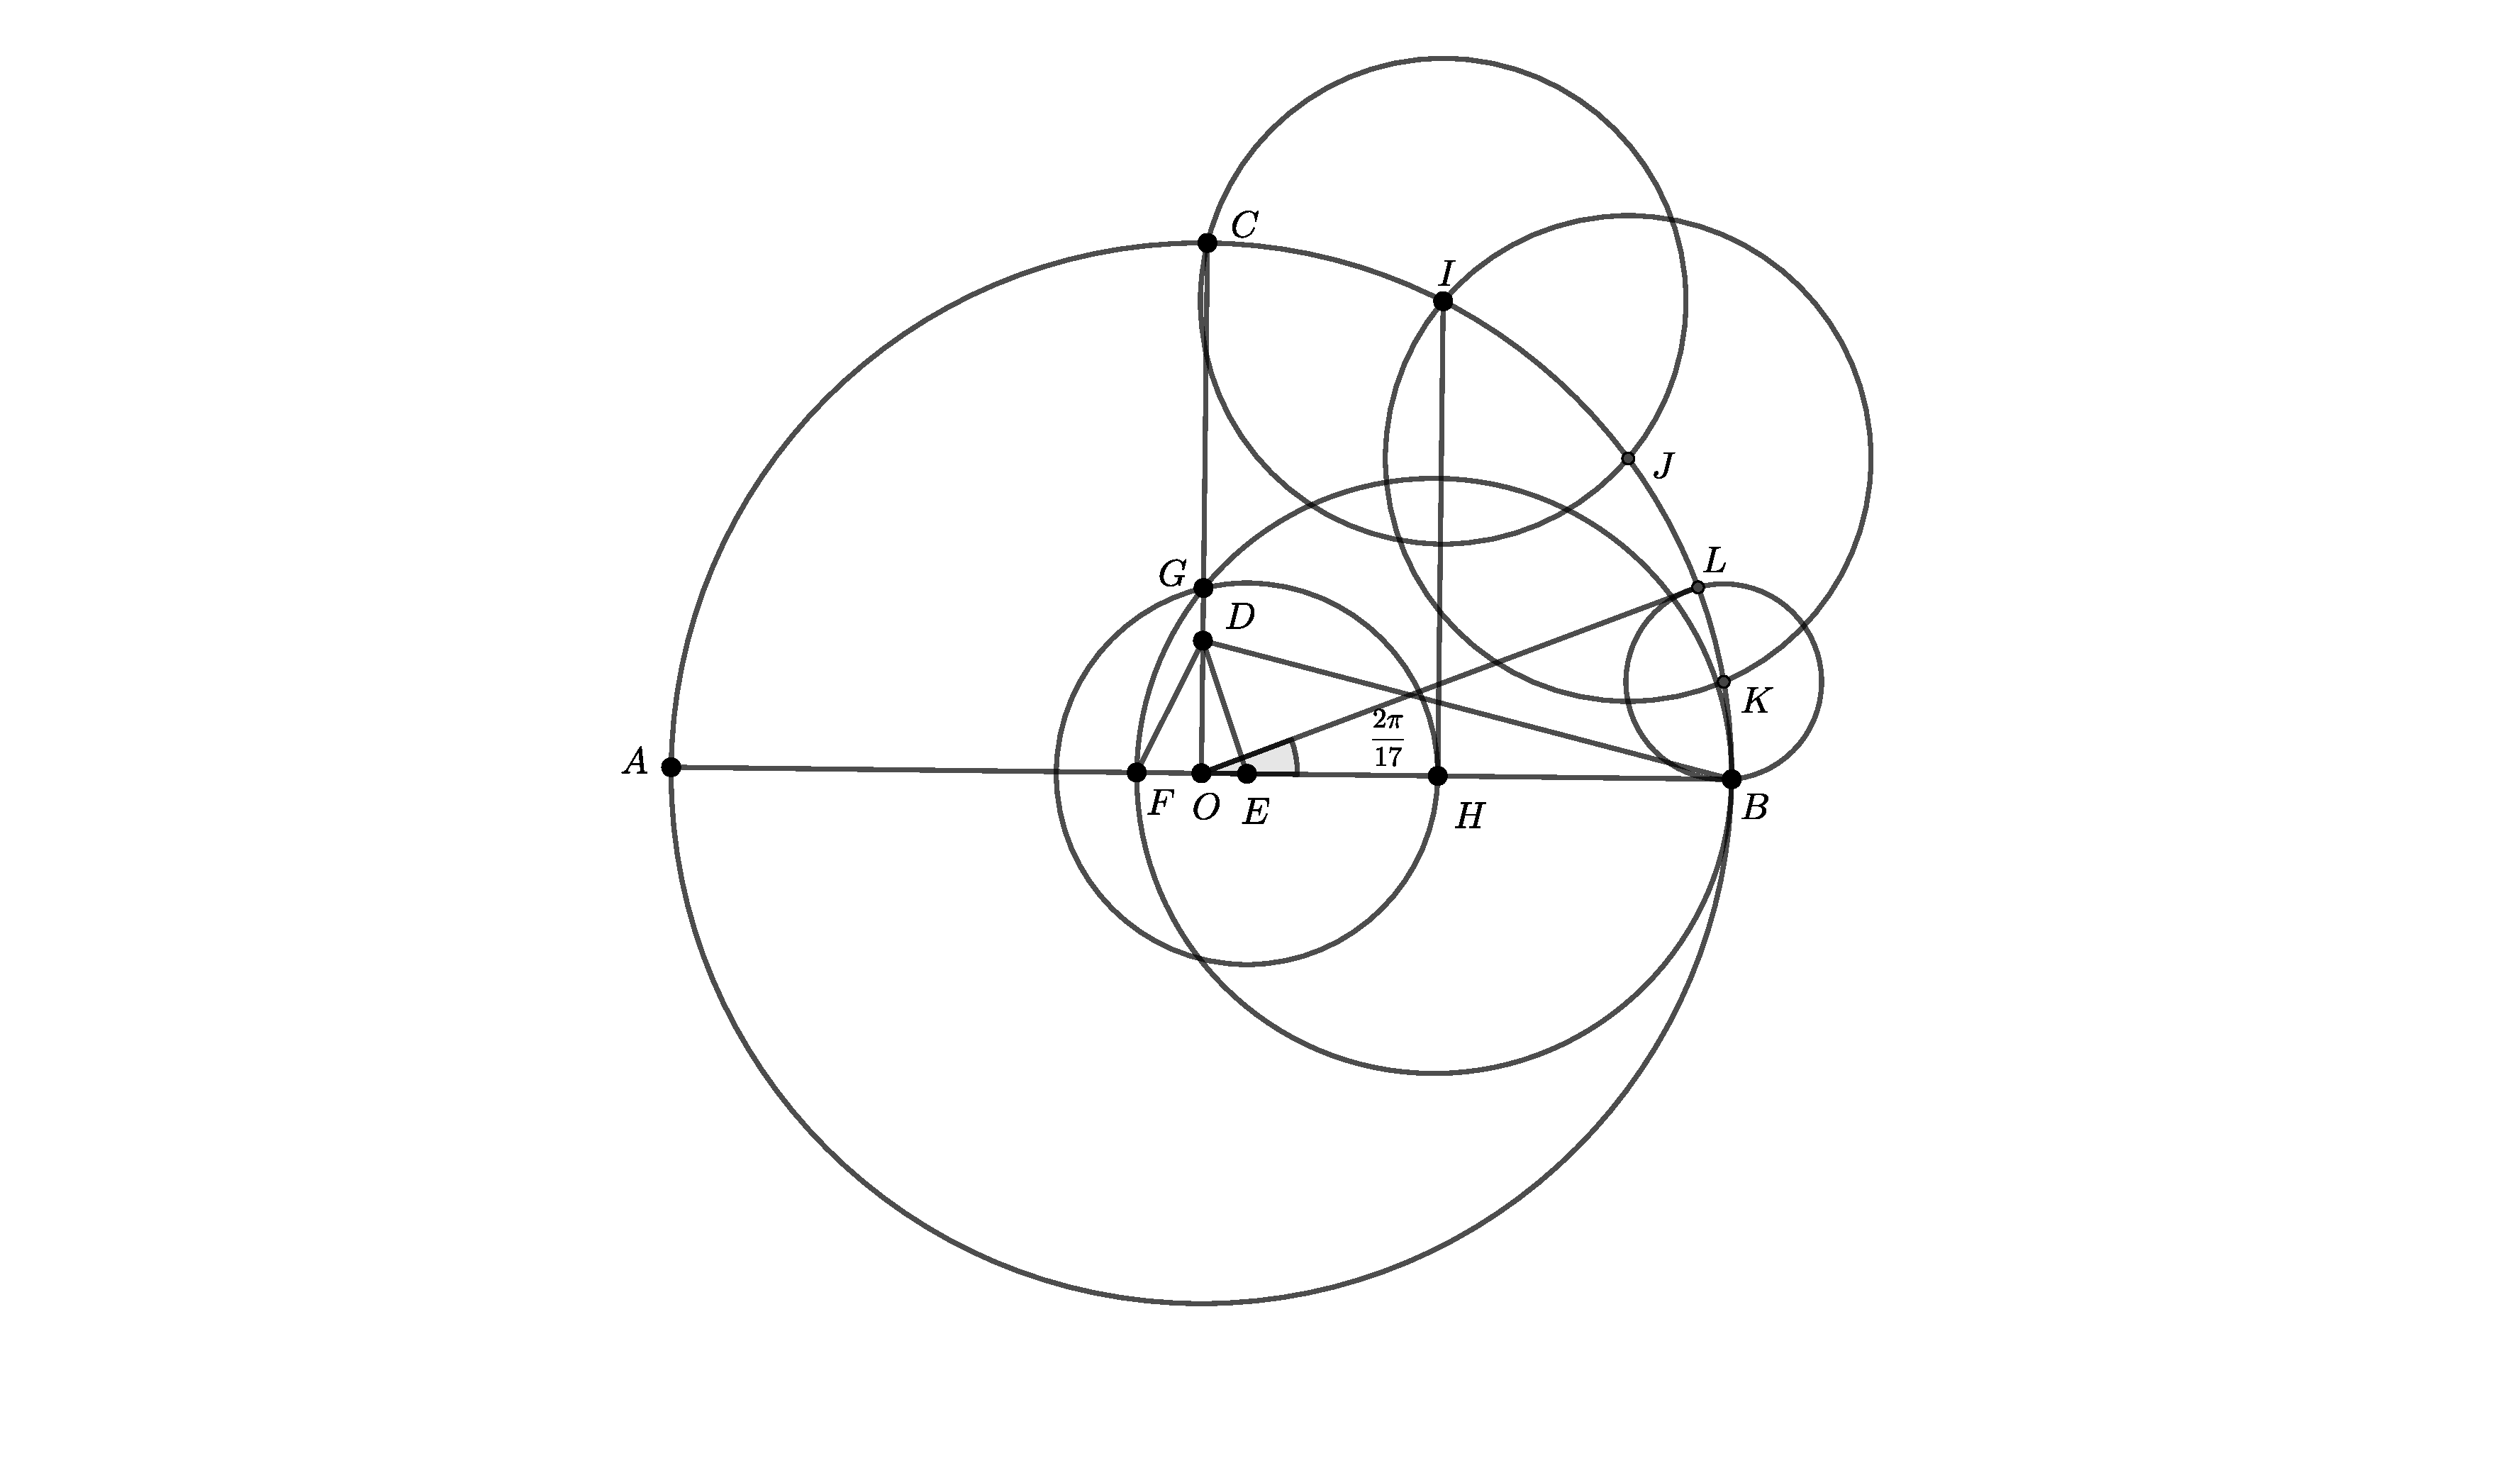
\includegraphics[scale = 0.3]{../figure/正17边形}
		\caption{正$17$边形}
	\end{figure}
	\begin{enumerate}
		\item 给定圆$O$,作直径$AB$;
		\item 作半径$OC$,使得$OC\perp AB$;
		\item 在线段$OC$上作点$D$,使得$OD=OC/4$;
		\item 在线段$OB$上作点$E$,使得$\angle ODE=\angle ODB/4$;
		\item 在线段$OA$上作点$F$,使得$\angle EDF=\pi/4$;
		\item 以线段$BF$为直径作圆,交线段$OC$于点$G$;
		\item 以点$E$为圆心,线段$EG$为半径作圆,交线段$OB$于点$H$;
		\item 过点$H$,作线段$AB$的垂线,交圆$O$于点$I$;
		\item 以点$I$为圆心,过点$C$作圆,交圆$O$于点$J$;
		\item 以点$J$为圆心,过点$I$作圆,交圆$O$于点$K$;
		\item 以点$K$为圆心,过点$B$作圆,交圆$O$于点$L$;
		\item 得到角$\angle BOL=2\pi/17$。
	\end{enumerate}
\end{problem}

\subsection{对称函数基本定理}

\begin{definition}{对称多项式 symmetric function}
	对于环$(R,+,\;\cdot\;)$,称多项式$f(x_1,\cdots,x_n)\in R[x_1,\cdots,x_n]$为对称多项式,如果对于任意置换$\sigma\in S_n$,成立%
	$$
	f(x_1,\cdots,x_n)=f(x_{\sigma(1)},\cdots,x_{\sigma(n)})
	$$
\end{definition}

\begin{definition}{初等对称函数 elementary symmetric function}
	$$
	s_k=\sum_{1\le i_1 < i_2 <\cdots <i_k \le n}x_{i_1}\cdots x_{i_k},\qquad 1\le k \le n
	$$
\end{definition}

\begin{lemma}
	对于域$K$,域扩张
	$$
	K(x_1,\cdots,x_n)/K(s_1,\cdots,s_n)
	$$
	为Galois扩张,其Galois群为$S_n$。
\end{lemma}

\begin{theorem}{对称函数基本定理 fundamental theorem on symmetric functions}
	对于域$K$上的多项式$f(x_1,\cdots,x_n)\in K[x_1,\cdots,x_n]$,成立%
	\begin{align*}
		&f(x_1,\cdots,x_n)\text{ 为对称多项式}\\
		\iff
		&\text{存在多项式 }g(x_1,\cdots,x_n)\in K[x_1,\cdots,x_n],\text{ 使得成立 }f(x_1,\cdots,x_n)=g(s_1,\cdots,s_n)
	\end{align*}
\end{theorem}

\begin{corollary}
	对于有限群$G$,存在Galois扩张$K/k$,使得成立$\text{Aut}_k(K)\cong G$。
\end{corollary}

\begin{corollary}
	对于域$K$,令%
	$$
	\Delta=\prod_{1\le i < j\le n}|x_i-x_j|
	$$
	那么域扩张%
	$$
	K(x_1,\cdots,x_n)/K(s_1,\cdots,s_n)(\Delta)
	$$
	为Galois扩张,其Galois群为$A_n$。
\end{corollary}

\subsection{多项式方程的根式可解性}

\subsubsection{根式扩张}

\begin{definition}{单根式扩张}
	称$n$次单扩张$k(\alpha)/k$为单根式扩张,如果$\alpha^n\in k$。
\end{definition}

\begin{definition}{根式扩张 radical extension}
	\begin{enumerate}
		\item 称有限扩张$K/k$为根式扩张,如果存在升链
		$$
		k=F_0\sub F_1\sub\cdots\sub F_{r-1}\sub F_r=K
		$$
		使得对于任意$1\le i \le r$,$F_{i}/F_{i-1}$为单根式扩张。
		\item 称域扩张$k(\alpha_1,\cdots,\alpha_r)/k$为根式扩张,如果对于任意$1\le i \le r$,存在$n_i\in\N^*$,使得成立$\alpha_i^{n_i}\in k(\alpha_1,\cdots,\alpha_{i-1})$。
	\end{enumerate}
\end{definition}

\begin{definition}{可解扩张 solvable extension}
	称域扩张$K/k$为可解扩张,如果存在根式扩张$F/k$,使得成立$K\sub F$。特别的,称Galois扩张$K/k$为可解的,如果$\text{Aut}_k(K)$为可解群。
\end{definition}

\begin{lemma}
	对于可分根式扩张$K/k$,存在Galois根式扩张$F/k$,使得成立$K\sub F$。
\end{lemma}

\begin{lemma}
	对于Galois扩张$K/k$,如果$\cha(k)=0$且$k$包含充分多的单位根,那么%
	$$
	K/k\text{ 为根式扩张}
	\iff
	K/k\text{ 为可解扩张}
	$$
\end{lemma}

\begin{proposition}
	对于Galois扩张$K/k$,如果$\cha(k)=0$,那么%
	$$
	K/k\text{ 为可解扩张}
	\iff
	\text{存在Galois根式扩张 }F/k,\text{ 使得成立 }K\sub F
	$$
\end{proposition}

\subsubsection{多项式的根式可解性}

\begin{definition}{一般多项式 general polynomial}
	对于特征为$0$的域$k$,$a_1,\cdots,a_n$为$k$上的未定元,称$k$上的$n$次一般多项式为$k(a_1,\cdots,a_n)$上的不可约多项式%
	$$
	f(x)=x^n+a_1x^{n-1}+\cdots+a_n
	$$
\end{definition}

\begin{definition}{多项式的Galois群}
	对于域$k$上的多项式$f(x)$,其分裂域为$K$,定义$f(x)$的Galois群为
	$$
	\text{Gal}_k(f(x))=\text{Aut}_k(K)
	$$
\end{definition}

\begin{definition}{根式可解 radical solvable}
	对于域$k$上的多项式$f(x)$,其分裂域为$K$,称$f(x)$在$k$中根式可解,如果存在根式扩张$F/k$,使得成立$K\sub F$。
\end{definition}

\begin{theorem}{一般多项式的Galois群}{一般多项式的Galois群}
	对于特征为$0$的域$k$上的$n$次一般多项式$f(x)$,成立%
	$$
	\text{Gal}_k(f(x))\cong S_n
	$$
\end{theorem}

\begin{theorem}{Galois准则 Galois' criterion}{Galois准则}
	对于特征为$0$的域$k$上的多项式$f(x)$,如果$f(x)$为不可约多项式,那么
	$$
	f(x)\text{在}k\text{上根式可解}\iff
	\text{Gal}_k(f(x))\text{为可解群}
	$$
\end{theorem}

\begin{theorem}{Abel-Ruffini定理}{Abel-Ruffini定理}
	对于特征为$0$的域$k$上的$n$次一般多项式$f(x)$,当且仅当$n\ge 5$时,$f(x)$在$k$上根式不可解。
\end{theorem}

\begin{proof}
	由定理\ref{thm:Sn的可解性}、\ref{thm:一般多项式的Galois群}与\ref{thm:Galois准则},命题得证!
\end{proof}

\vspace{2.1cm}

\begin{center}
	{\large\kaishu 我希望终将会有智者能从这混沌之中受益匪浅。}
\end{center}

\begin{flushright}
	--- {\large\fontspec{EB Garamond} Evariste Galois}
\end{flushright}

% \end{document}
